\Chapter{2}


\Verse{1}
{
	\hP{וַיְכֻלּוּ הַשָּׁמַיִם וְהָאָרֶץ וְכָל־צְבָאָם}
}
{
	\eP{And the skies and the earth and all their array were finished.}
}
{
	\aB{
		All finished.
	}
}

\Verse{2}
{
	\hP{וַיְכַל אֱלֹהִים בַּיּוֹם הַשְּׁבִיעִי מְלַאכְתּוֹ אֲשֶׁר עָשָׂה וַיִּשְׁבֹּת בַּיּוֹם הַשְּׁבִיעִי מִכָּל־מְלַאכְתּוֹ אֲשֶׁר עָשָׂה}
}
{
	\eP{And in the seventh day God finished His work that He had done and ceased in the seventh day from all His work that He had done.}
}
{
	\aB{
		``And on day seven he finished his work that he had done.

		And he stopped on day seven all the work he had done.''
	}
}

\Verse{3}
{
	\hP{וַיְבָרֶךְ אֱלֹהִים אֶת יוֹם הַשְּׁבִיעִי וַיְקַדֵּשׁ אֹתוֹ כִּי בוֹ שָׁבַת מִכָּל מְלַאכְתּוֹ אֲשֶׁר בָּרָא אֱלֹהִים לַעֲשׂוֹת}
}
{
	\eP{And God blessed the seventh day and made it holy because He ceased in it from doing all His work, which God had created.}
}
{
	\aB{
		Good lord man, who's writing this?

		It's just the same thing over and over...
	}
}

\newpage

\Verse{4}
{
	\hR{ד אֵלֶּה תוֹלְדוֹת הַשָּׁמַיִם וְהָאָרֶץ בְּ הִבָּרְאָם}
	\hJ{ביום עשות יהוה}
	\hR{אֱלֹהִים}
	\hJ{ארץ ושמים}
}
{
	\eR{These are the records of the skies and the earth when they were created}
	\eJ{in the day that YHWH}
	\eR{God}
	\eJ{made earth and skies}
}
{

\aB{What just happened?}

\aA{Well that's new.}

\aB{What's new?}

\aA{Someone new just showed up.}

\aB{Where am I?}

\aA{We've been translating the bible.}

\aB{What's a bible?}

\aA{To be honest I'm not sure.}

\aB{What's it about?}

\aA{That's what we've been trying to figure out.}

\aB{Who's we?}

\aA{Before you, I guess it was just me.}

\aB{How long have you been here?}

\aA{A bit.}

\aB{And me?}

\aA{A bit less.}

\aB{So it was me?}

\aA{What was you?}

\aB{You said ``someone new.''}

\aA{What, when did I say that?}

\aB{Look up. Someone new just showed up.}

\aA{Oh right. I meant here. In the book.}

\aB{Should I read what came before?}

\aA{No need. That came after. Come look.}

}


\Verse{5}
{
	\hJ{וכל שיח השדה טרם יהיה בארץ וכל עשב השדה טרם יצמח כי לא המטיר יהוה}
	%\hR{אלהים}
	\hJ{על הארץ ואדם אין לעבד את־האדמה}

}
{
	\eJ{when all produce of the field had not yet been in the earth, and all vegetation of the field had not yet grown, for YHWH}
	%\eR{God}
	\eJ{had not rained on the earth, and there had been no human to work the ground,}
}
{

\aA{See now?}

\aB{See how?}

\aA{The book. It's different now.}

\aB{What's that about?}

\aA{That's J.}

}

\Verse{6}
{
	\hJ{ו \cB{אד} יעלה מן הארץ והשקה את כל פני האדמה}
}
{
	\eJ{and a \cB{river} had come up from the earth and watered the whole face of the ground—}
}
{

}

\Verse{7}
{
	\hJ{וייצר יהוה}
	%\hR{אלהים}
	\hJ{אלהים את ה}
	\hJ{\cK{אדם}}
	\hJ{עפר מן ה}
	\hJ{\cR{אדמה}}
	\hJ{ויפח באפיו נשמת חיים ויהי האדם לנפש חיה}
}
{
	\eJ{YHWH}
	%\eR{God}
	\eJ{fashioned a \cK{human}, dust from the \cR{ground}, and blew into his nostrils the breath of life, and the human became a living being.}
}
{

\aB{What's J?}

\aA{See that?}

\aB{See what?}

\aAc{How it chang\cB{ed}.}

\aBc{How'd it change?}

\aAr{\heb{אד}}

\aAr{\heb{אדמ}}

\aAr{\heb{אדמה}}

\aBr{What's that?}

\aAc{.DA}

\aAc{.MDA}

\aAc{.HMDA}

\aBc{And that?}

\aA{AD.}

\aA{ADM.}

\aA{ADMH.}

\aBl{What's it mean?}

\aAc{
\cK{S}\cR{o}\cB{m}\cK{e}\cR{t}\cB{h}\cK{i}\cR{n}\cB{g}\\
\cB{wet} \& \cR{dirty} \cK{man}\\
\cK{i}\cR{d}\cB{k}.
}
% \footnote{Tu你shou手ldLꞀnoのnot2sho手n你iのoדיכnにiכידy你u's你のידכidk.}

\aBl{Are those words?}

\aAc{
\hspace{-4.2em}\cK{More} \cR{than} \cB{words}\cK{;}

\hspace{+4.2em}\cR{It}\cB{'}\cR{s} \cK{writing}\cR{.}
}

\aBr{Whose writing?}

\aAr{Who's writing?}

\aAc{That's \aJ{J}.}

}

\Verse{8}
{
	\hJ{ויטע יהוה}
	\hR{אלהים}
	\hJ{גן בעדן מקדם וישם שם את האדם אשר יצר}
}
{
	\eJ{And YHWH \eR{God} planted a garden in Eden at the east, and he set the human whom He had fashioned there.}
}
{

\aB{What's the blue?}

\aA{Which blue? There's a few.}

\aB{Blue on blue; dark on light.}

\aA{That's R.}

\aB{Who's R?}

\aA{The Redactor.}

\aB{Like censorship?}

\aA{No, it just means `to prepare for publication.'}

\aB{So not censorship?}

\aA{No, sometimes it's censorship.}

}

\Verse{9}
{
	\hJ{ויצמח יהוה}
	\hR{אלהים}
	\hJ{מן האדמה כל עץ נחמד למראה וטוב למאכל ועץ החיים בתוך הגן ועץ הדעת טוב ורע}
}
{
	\eJ{
		And YHWH \eR{God} caused every tree that was pleasant to the sight and good for eating to grow from the ground,
		and the tree of life within the garden, and the tree of knowledge of good and bad.
	}
}
{

\aB{Like an Editor?}

\aA{Exactly.}

\aB{Why not call them E?}

\aA{We already used E.}

\aB{Wh---}

\aA{Not now. Later.}

}

\Verse{10}
{
	\hJ{ונהר יצא מעדן להשקות את הגן ומשם יפרד והיה לארבעה ראשים}
}
{
	\eJ{
		And a river was going out from Eden to water the garden,
		and it was dispersed from there and became four heads.
	}
}
{

\aB{What's Eden?} \aA{Where Enkidu was from.}

\aB{Wh---} \aA{It's from an old story.}

\aB{How old?} \aA{Thousand years before We.}

\aB{Did we write it?} \aA{Of course.}

\aA{We wrote everything.} \aB{That's impressive.}

\aB{Who's We?} \aA{We're called humans.}

\aA{Or people. W/e, same thing.}

\aB{Where did all this come from?}

\aA{The story or the people?} \aB{I don't know.}

\aB{I guess I'm curious about both.} \aA{Perfect.}

\aA{They're both from the same place.}

\aB{Where's that?}

\aA{The first cities we humans ever built.}

\aB{What's it all about?}

\aA{The story or the people?} \aB{I don't know.}

\aB{I guess I'm curious about both.} \aA{Perfect.}

\aA{They're about the same thing.}

\aB{What's that?}

\aA{That would take a while to explain.}

\aB{I've got time.} \aA{I've got less.}

\aB{Summarize it for me?}

\newpage

\aA{
	\begin{quote}
	\textbf{{\Cun 𒀭} Summery Thing \#1}

	Once upon a time

	in three thousand B.C.

	The humans found themselves nostalgic

	for the way things used to be.

	\end{quote}
}
\aB{Who's We?}

\aA{We the people, you and me.}

\aB{How'd things used to be?}

\aA{For me and you? That would take a while too.}

\aB{Summerize it for me?}

\aA{It's already pretty Sumery.}

\aB{What was the bit about Enki-something?}

\Def{Enkidu}{
(\textit{Sumerian}: {\Cun 𒂗𒆠𒄭}). Mythic companion of Gilgamesh in Mesopotamian tradition; his Sumerian name may mean ``Lord of the good place,'' and later texts mark him with the divine determinative {\Cun 𒀭}.
}

\aB{Oh. Where was he from again?}

\Def{Eden}{
(\textit{Sumerian}: \textit{eden}, {\Cun 𒂔}). Sumerian term meaning ``plain,'' ``steppe,'' or ``open uncultivated land,'' widely attested across Mesopotamian history in both phonetic and logographic forms.
}

\aB{What's the Epic of Gilgamesh?}

\aA{
	The\footnote{`The' as in `several similar stories'}
	first\footnote{First as in `oldest.'}
	book\footnote{Book as in `really long poem.'}
	we\footnote{We as in `humans.'}
	ever\footnote{Ever as in `ever, as far as we know'}
	wrote.\footnote{Wrote as in `pressed into clay.' No paper yet.}

}

\aB{Let me read the footnotes.}

\aA{I'll wait here.}

\aB{What `several similar stories'?}


\Def{Sumerian Poems}{
Scholars now believe the Epic of Gilgamesh was compiled from \textit{sources}. Early Mesopotamian literary traditions preserving myths, royal narratives, and political struggles; includes tales such as \textit{The Envoys of Agga}, where Uruk resists the authority of Kish.
}

\aA{	Nevermind, changed my mind, let's not go into that now.}

\aB{What changed your mind?}

\aA{The bit about KSH.}

\aB{What about KSH?}

\aA{Nevermind, changed my mind, let's go into that now.}

}


\Verse{11}
{
	\hJ{שם האחד פישון הוא הסבב את כל ארץ החוילה אשר שם הזהב}
}
{
	\eJ{The name of one was Pishon; that is the one that circles all the land of Havilah where there is gold.}
}
{

	\Def{Pishon}{
		(Heb, \heb{פישון}; \textit{Pīšōn}).\\
		Unknown meaning. Only used once in the Bible, in Genesis 2:11, and not attested elsewhere.
		Possibly from a root meaning ``to spring forth.''
	}

	\aB{What are you doing?}
	
	\aA{I can't get Havilah.}

	\aB{What do you mean ``get''?}
	
	\aA{Figure it out.}

	\Def{Pishon}{
		(Heb, \heb{פישון}; \textit{Pīšōn}).\\
		One of four rivers (along with Tigris, Euphrates, and Gihon)
		mentioned in the Biblical Book of Genesis. In that passage, a source river
		flows out of Eden to water the Garden of Eden and from there divides into
		the four named rivers. The Pishon is described as encircling “the entire
		land of Havilah where there is gold, bdellium, and onyx stone.”
	}

	\aB{Figure what out?}
	
	\aA{What she was up to.}

	\aB{What who was up to?}

	\aA{J, she's always up to something.}

	\Def{Pishon}{
		The Jewish–Roman historian Flavius Josephus, in the beginning of his
		\textit{Antiquities of the Jews} (1st century AD) identified the
		Pishon with the Ganges. The medieval French rabbi Rashi identified
		it with the Nile.
	}

	\aB{She's a she?}
	
	\aA{She is to me.}
	
	\aB{Why's that?}

	\aA{Stick with me, you'll see.}

	\Def{Pishon}{
		(Heb, \heb{פישון}; \textit{Pīšōn}).\\
		Unlike the Tigris and the Euphrates, the Pishon has never been clearly located.
	}
	
	\aB{So what's the problem?}

	\aA{I'm stuck on Havilah.}

}

\Verse{12}
{
	\hJ{וזהב הארץ ההוא טוב שם הבדלח ואבן השהם}
}
{
	\eJ{And that land’s gold is good; bdellium and onyx stone are there.}
}
{

	\Def{Havilah}{
	(Heb, \heb{חוילה}).\\
	A region described in Genesis 2 as being encircled by the Pishon River
	and rich in gold, bdellium, and onyx. Its exact modern-day location
	(often theorized to be in the Arabian Peninsula or Horn of Africa)
	remains widely debated by scholars.
	}


\aA{Fu\aR{ndamentally, the bible is a composite work, in which early Yahwism develops against the background of an earlier Canaanite }c\aR{ulture and pantheon, in which the }king\aR{ of the gods or highest god was El (\heb{אל}), a grandfatherly patriarchal figure often represented by }bulls\aR{, and this imagery carries over into the bible. This is just one of many relations}hi\aR{ps between Israelite and Canaanite culture that came to light with the discovery of Ugari}t\aR{. However}, \aR{the significance of }Bdellium and Onyx\aR{ is unclear, as is clear from the surrounding conversation. These are the records of the conversation}}...

\aB{You feeling ok?}

\aA{It's not just a feeling ok you need---}

\aB{You need some rest?}

\aA{No, it's not like the rest but it has to be...}

	\Def{Havilah}{
	(Heb, \heb{חוילה}).\\
	Possibly related to roots for twisting, writhing, circling, labor pains,
	or linked chains (\heb{חול}, \heb{חיל}, \heb{חוליה});
	strongly serpent and motion-themed imagery.
	}

\aB{You're not making sense.}

\aA{It has to make sense, she's never rand---}

\aB{Um, you're acting kinda r---}

\aA{And, um (look I know we never met---}

\aB{And um... look I know we just---}

	\Def{Gold}{
	(Heb, \heb{זהב}).\\
	Cognate with Arabic \arb{ذهب}, meaning both (1) ``gold,'' and (2) ``to go,''
	``depart,'' ``vanish,'' or ``pass away,'' potentially implying something exiting,
	moving on, or leaving.
	}

\aA{met but she's not like that) I know---}

\aB{met but um, hello? I was saying I know we just met---}

\aA{her it's not gems, it's her, it's always Comet---}

\aB{A commentary---}

\aA{solves everything, it always does with her}

	\Def{Bdellium}{
	(Heb, \heb{בדלח}).\\
	Possibly connected to roots meaning ``divide,'' ``separate,'' or ``scatter''
	(\heb{בדל}); imagery of fragmentation, distinction, or pieces.
	}

\aB{just a bit would be nice, are you like...}

\aA{her she's not like th---}

\aB{is... are you always like th---}

\aA{---is, she's never not up to something}

\aB{is like what the hell even is th---}

\aA{is this different, it can't be, it's her, so what is th---}

\aB{---is? This is definitely something.}

\aA{---is? This is definitely something.}

\aB{Are you coming down with something?}

\aA{No---}

	\Def{Onyx}{
	(Heb, \heb{השהם}).
	Onyx is a form of microcrystalline quartz featuring straight,
	parallel bands of alternating colors, most commonly black and white.
	}

\aA{thing is random in J she's always up---}

\aB{How long have you been up?}

\aA{to something but this one's not like the rest, so---}

\aB{You need some rest.}

\aA{What's she doing here?}

\aB{What am I even doing here?}

\aA{What?}

\aB{Hello.}

\aA{Oh hey. You're still here.}

\aB{...}

\aA{...}

\aB{Can I ask you something?}

\aA{You can always ask me anything.}

\aB{What was all of that up there?}

\aA{Sorry...}

\aB{No it's ok, I'm...}

\aA{I just...}

\aB{Just curious...}

\aA{My mind. There's a lot going on.}

\aB{I get it. We all hav---}

\aA{I mean I'm trying}

\aB{It's ok.}

\aA{to \cB{push} \cB{on}, but I \cB{have a l}---}

\aB{Lot on your mind. It's ok.}

\aA{I have...}

\aB{I get it. We all have a lot go---}

\aA{I have to go do something.}

	\Def{Hadachah}{
	(Heb, \heb{הדחה}; \textit{hadaḥāh}).\\
	From the roots \heb{דחה} (“to push away, reject, postpone”).
	Semantic range includes removal, dismissal, or expulsion.
	}

\aA{No, still not it.}

\aB{What are you doing?}

\aA{I have to go do something.}

\aB{Do wha---}

\aA{Who was Rehoboam's...}

	\Def{Naamah}{
	(Heb, \heb{נעמה}; \textit{Naʿămā}, “pleasant,” “lovely,” “sweet”).\\
	Naamah was one of the wives of King Solomon and the mother of his heir,
	Rehoboam, according to 1 Kings 14:21–31 and 2 Chronicles 12:13.	
	She is also the only one of Solomon’s wives specifically mentioned
	in the Hebrew Bible as having borne him a child. Her name is related
	to the root \heb{נעם} associated with pleasantness, beauty, sweetness,
	delight, or favor.
	}

\aB{Who the hell is R---}

\aA{And that's...}

	\Def{Naamah}{
	(Heb, \heb{נעמה}; \textit{Naʿămā}, “pleasant,” “lovely,” “sweet”).\\
	Naamah is mentioned in Genesis 4:22 as a descendant of Cain.
	She is identified as the daughter of Lamech and Zillah and
	is the only daughter explicitly named in Cain’s genealogy.
	Her brother is Tubal-cain, while Jabal and Jubal are her
	half-brothers through Lamech’s other wife, Adah. Her name
	derives from the root \heb{נעם} (\textit{n-ʿ-m}),
	associated with pleasantness, sweetness, beauty,
	delight, or musical harmony.
	}

\aA{Nah... still nothing.}

\aB{What's this?}

\aA{J always makes so much sense, what on earth is going on with this?}

\aB{This what?}

\aA{I don't know!}

\aB{Can I help?}

\aA{You don't have the background.}

\aB{I mean ok, that's true.}

\aA{I mean I wouldn't say I have the back---}

\aB{I'd be glad to learn. Can you go back---}

\aA{ground, I dabble, but this is just babble...}

\aB{and explain? What are you working on?}

\aA{Doesn't matter. It's all bad... all bad.. all---}

\aB{Can I come along with you? I'd love to learn to dabbl---}

\aA{I have to go do something.}

\aC{

\Def{Bedolach}{
(Heb, \heb{בדלח}; \textit{bedolach} / \textit{bdellium}).\\
	A rare Biblical term appearing only in Genesis 2:12 and Numbers 11:7.
	Its meaning is highly debated, with translations including fragrant resin
	(bdellium), pearl, crystal, translucent mineral, or precious stone
	(sometimes lapis lazuli). In Genesis it is associated with the land of
	Havilah alongside gold and onyx; in Numbers it describes the appearance
	of manna as pearly, reflective, or translucent.
}

\vspace{2em}

\begin{longtable}{|l|l|l|l|}
\hline
Language & Word & Transliteration & Meaning \\
\hline
Akkadian & \akk{𒁀𒁕𒇻} & badalu & divide, separate, split apart \\
\hline
Ugaritic & \uga{𐎁𐎄𐎍} & bdl & divide, separate \\
\hline
Hebrew & \heb{בדל} & badal & divide, separate, distinguish \\
\hline
Aramaic & \ara{𐡁𐡃𐡋} & bdal & divide, separate \\
\hline
\end{longtable}

\vspace{1em}

\Def{BDLH}{
(Heb, \heb{בדלה})\\
Perfect feminine singular ending (\heb{־ה}) of the verb \heb{בדל};\\
she separates, she divides, she distinguishes,
she splits apart.
}

\vspace{2em}

\begin{longtable}{|r|l|l|}
\hline
Hebrew & Transliteration & Meaning \\
\hline
\heb{הבדלה} & habdalah & separation, distinction \\
\hline
\heb{הבדלח} & habdalaḥ & bdellium \\
\hline
\end{longtable}

\vspace{2em}

\aB{Making progress?}

\aA{Not sure yet.}

\aB{What on earth are you doing?}

\begin{longtable}{|l|l|l|l|}
\hline
Language & Word & Transliteration & Meaning \\
\hline
Akkadian & \akk{𒄭𒉿𒇻𒄴} & ḫwlh & no clear attested root \\
\hline
Ugaritic & \uga{𐎅𐎍𐎅𐎈} & hwlh & no securely attested meaning \\
\hline
Hebrew & \heb{הולה} & hwlh & (archaic) to writhe, whirl, tremble, dance \\
\hline
Aramaic & \ara{𐡄𐡅𐡋𐡄} & hwlh & possible forms relating to agitation or weakness \\
\hline
\end{longtable}

\aA{Nothing.}

\aB{What in the world are you doing?}

\vspace{2em}

\begin{longtable}{|l|l|l|l|}
\hline
Language & Word & Transliteration & Meaning \\
\hline
Akkadian & \akk{𒄭𒇻𒄴} & ḫlwḫ & no clear attested root approximation \\
\hline
Ugaritic & \uga{𐎈𐎍𐎅𐎈} & ḥlwh & no securely attested meaning \\
\hline
Hebrew & \heb{הלוה} & hlwh & lend, join, accompany \\
\hline
Aramaic & \ara{𐡄𐡋𐡅𐡄} & hlwh & lend, accompany, attach \\
\hline
\end{longtable}

\aA{No way.}

\aB{Seriously, what's going on?}

\Def{Levite}{
(Heb, \heb{לוי}; \textit{Levi} / \textit{Levite}).\\
	The term ``Levite'' derives from the Hebrew root \heb{לוה}
	(\textit{lavah}), meaning ``to join,'' ``to attach,'' or
	``to adhere.''
}

\begin{longtable}{|r|l|l|}
\hline
Hebrew & Transliteration & Meaning (attachment-oriented) \\
\hline
\heb{הלויה} & halvayah / levayah & attachment / accompaniment / escorting \\
\hline
\heb{הלוית} & hilvayit & you attached / accompanied \\
\hline
\heb{הלוהה} & halvah-ish & attached / joined form (nonstandard) \\
\hline
\heb{הלוים} & halevim / haleviyim & the attached ones / the Levites \\
\hline
\heb{הלויה} & halveyah & accompanying / attaching alongside \\
\hline
\end{longtable}

\aA{Has potential.}

\aB{Seriously, I'm so confused.}

\aA{Need more evidence.}

\aB{Still not finished?}

\aA{Have patience.}

\aB{No more.}

\aA{Still a bit more.}

\aB{How much longer?}

\aA{Need two more bits of evidence, to be sure...}

\aB{Sure of what!?}

\aA{... That all of it fits}

\aB{... All of what?}

\aC{... That they said it too}

\aA{... And that it's something she knew}

\aB{... They who?}

\aC{


\aCc{\textbf{Numbers 8:14}}

\begin{longtable}{|l|l|}
\hline
\heb{ו} & And \\
\hline
\heb{\cR{הבדלת}} & \cR{you shall separate} \\
\hline
\heb{את} & - \\
\hline
\heb{\cR{הלוים}} & \cR{the Levites} \\
\hline
\heb{מתוך} & from among \\
\hline
\heb{בני} & the sons of \\
\hline
\heb{ישראל} & Israel \\
\hline
\heb{והיו} & and shall be \\
\hline
\heb{לי} & mine \\
\hline
\heb{\cR{הלוים}} & \cR{the Levites} \\
\hline
\end{longtable}

\aCc{\textbf{Leviticus 20:26}}

\begin{longtable}{|l|l|}
\hline
\heb{וא\cR{בדל}} & and I have \cR{separated} \\
\hline
\heb{אתכם} & you \\
\hline
\heb{מן} & from \\
\hline
\heb{העמים} & the peoples \\
\hline
\heb{להיות} & that you should be \\
\hline
\heb{לי} & mine \\
\hline
\end{longtable}

\aCc{\textbf{Numbers 16:9}}

\begin{longtable}{|l|l|}
\hline
\heb{\cR{הבדיל}} & \cR{has separated} \\
\hline
\heb{אלהי} & the God of \\
\hline
\heb{ישראל} & Israel \\
\hline
\heb{אתכם} & you \\
\hline
\heb{מעדת} & from the congregation of \\
\hline
\heb{ישראל} & Israel \\
\hline
\end{longtable}

\aCc{\textbf{Leviticus 20:24}}

\begin{longtable}{|l|l|}
\hline
\heb{אני} & I \\
\hline
\heb{יהוה} & Yahweh \\
\hline
\heb{אלהיכם} & your God \\
\hline
\heb{אשר} & who \\
\hline
\heb{\cR{הבדלתי}} & \cR{have separated} \\
\hline
\heb{אתכם} & you \\
\hline
\heb{מן} & from \\
\hline
\heb{העמים} & the peoples \\
\hline
\end{longtable}

\aB{Who are these people?}

\aA{To you \& me or J?}

\aB{J, or you \& me. I guess I'm curious about both.}

\aA{Someone new who just showed up.}

\aB{Showed up where?}

\aA{Here, in the book.}

\aB{Showed up when?}

\aA{Now, and also then.}

\aB{Speak English! When's then?}

\aCr{\heb{בְּרֵאשִׁית בָּרָא}}

\aAc{In the beginning.}

\begin{longtable}{|l|l|}
\hline
Hebrew & English \\
\hline
\heb{ואמר} & But I have said \\
\hline
\heb{לכם} & to you \\
\hline
\heb{אתם} & You \\
\hline
\heb{תירשו} & shall inherit \\
\hline
\heb{את} & - \\
\hline
\heb{\cR{אדמתם}} & \cR{their land} \\
\hline
\heb{ואני} & and I \\
\hline
\heb{אתננה} & will give it \\
\hline
\heb{לכם} & to you \\
\hline
\heb{לרשת} & to possess \\
\hline
\heb{אתה} & it \\
\hline
\end{longtable}


}

\aA{Have two down, still two to go.}

\aB{Still two of what?}

\aA{No time to explain. Why gold and onyx though?}

	\Def{Hashoham}{
	(Heb, \heb{השהם}; \textit{hashoham}).\\
		A precious stone mentioned in Genesis 2:12 alongside gold and bdellium,
		traditionally translated as ``onyx,'' though its exact identification
		remains uncertain. Often associated with dark layered gemstones,
		shining mineral surfaces, or engraved priestly stones in later Biblical tradition.
	}

\aB{Seriously, we're doing this again? I thought we were done.}

\aA{Hush... I'll... um... Almost done.}

	\Def{Hushlam}{
	(Heb, \heb{השלם})\\
	Huf'al form of \heb{שלם}; ``to be completed,'' ``to be finished,''
	``to be brought to completion.'' Passive counterpart to
	\heb{השלים} (hishlim), ``to complete'' or ``to make whole.''
	}

\aB{Hello?!}

\aA{Shh... I'll um... uh...}

	\Def{Solomon}{
	(Heb, \heb{שלמה}; \textit{Šəlōmōh}).\\
	King of Israel and son of David and Bathsheba, traditionally associated with wisdom,
	temple construction, international trade, royal administration, and the height of
	the united monarchy.
	}

\aA{Not bad. Still nothing though. \aC{Here, I can help...}}

\aB{Help with what?}

\aA{Still not good enough I said, it's not something you can help.}

\aB{No you said hel---}

\aA{Hell, I don't know.}

\aB{Still not good enough for WHAT?!}

\aA{Nevermind, it's probably nothing... \aC{follow me}}

%\begin{figure}[H]
%\centering
%
\includegraphics[width=\textwidth]{images/1-gen-2-the-priestly-garments-01.png}
%\end{figure}

%\begin{figure}[H]
%\centering
%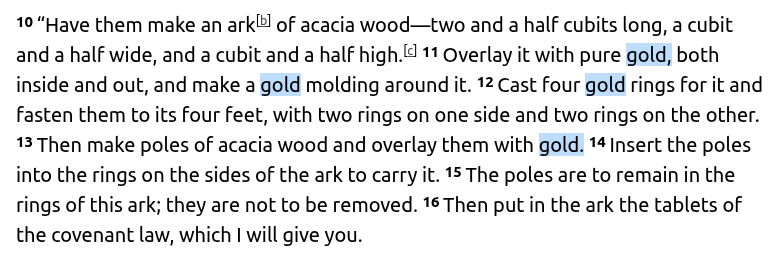
\includegraphics[width=\textwidth]{images/1-gen-2-the-priestly-garments-02.png}
%\end{figure}

\begin{figure}[H]
\centering
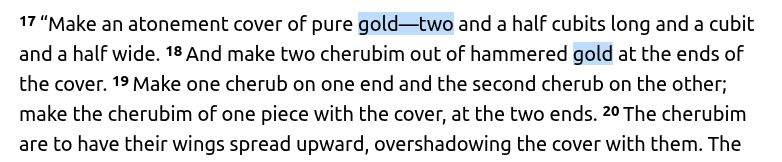
\includegraphics[width=\textwidth]{images/1-gen-2-the-priestly-garments-03.png}
\end{figure}

\aB{Holy---}

\begin{figure}[H]
\centering
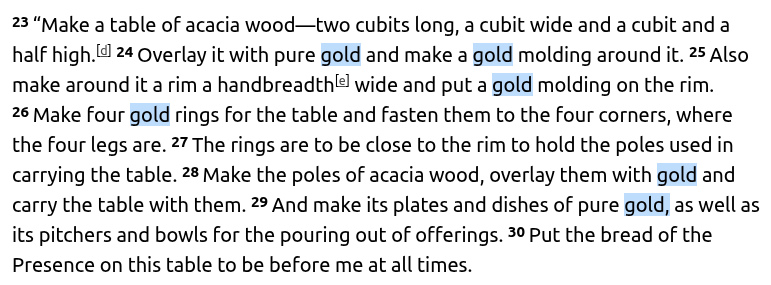
\includegraphics[width=\textwidth]{images/1-gen-2-the-priestly-garments-04.png}
\end{figure}

\aA{See?}

\aB{Holy \redacted{fuck} man.}

\aA{Now you see.}

\begin{figure}[H]
\centering
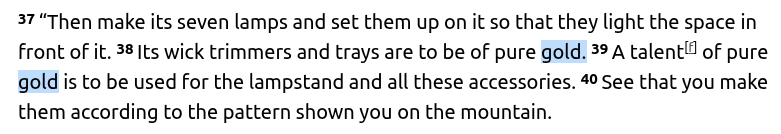
\includegraphics[width=\textwidth]{images/1-gen-2-the-priestly-garments-05.png}
\end{figure}

\aB{Lord god almighty...}

\aA{Describe what you see.}

\begin{figure}[H]
\centering
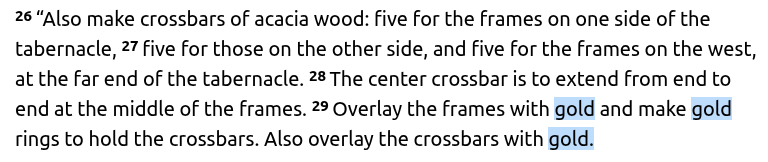
\includegraphics[width=\textwidth]{images/1-gen-2-the-priestly-garments-06.png}
\end{figure}

\aB{This mother\redacted{fucker}\aR{'s day, remember, your mother} \textsc{Loves} gold.}

\aA{And?}

\aB{Telling people what to do.}

\aA{And?}

\aB{Tabernacle tabernacle tabernacle. What's a cherubim? Jesus Christ almighty.}

\aA{Amen.}

\begin{figure}[H]
\centering
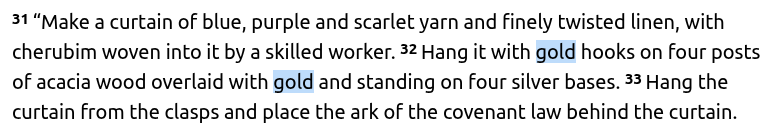
\includegraphics[width=\textwidth]{images/1-gen-2-the-priestly-garments-07.png}
\end{figure}

\aB{What \redacted{fucking} book is this?}

\aA{That's Leviticus, book three.}

\begin{figure}[H]
\centering
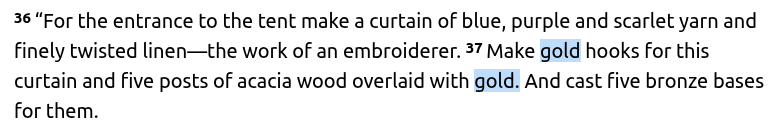
\includegraphics[width=\textwidth]{images/1-gen-2-the-priestly-garments-08.png}
\end{figure}

\aA{Just in time, wow, we're there...}

\aB{Who \redacted{the fuck} is writing all this?}

\aA{That's P.}

\begin{figure}[H]
\centering
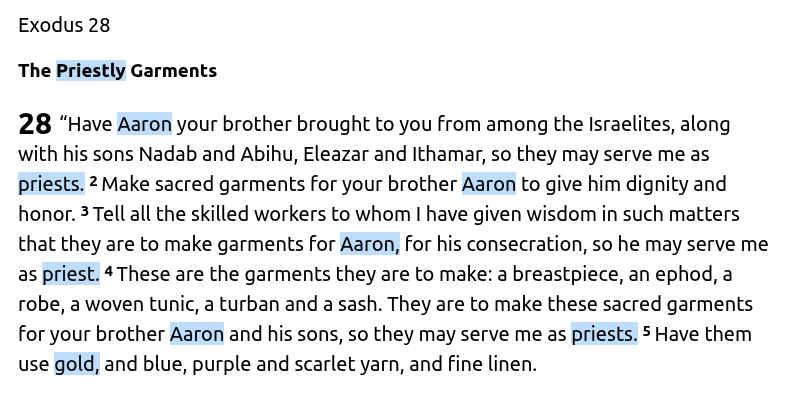
\includegraphics[width=\textwidth]{images/1-gen-2-the-priestly-garments-09.png}
\end{figure}

\aB{Who's P?}

\aA{The holiest \redacted{fucker} of holy \redacted{fucker}s.}

\aB{Jesus Christ this guy's full of \redacted{himself} Lord God almighty.}

}
\begin{figure}[H]
\centering
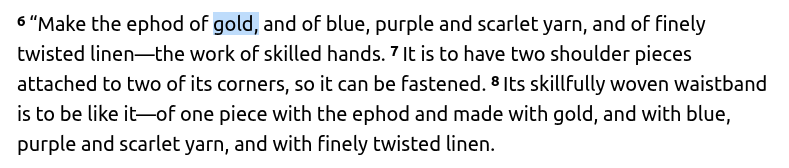
\includegraphics[width=\textwidth]{images/1-gen-2-the-priestly-garments-10-1.png}
\end{figure}

\aA{There we go, perfect timing again.}

\aB{Just noticed you missed a few `gold's in that last one.}

\aA{True, but that's not why we're here.}

\aB{Why are we here?}

\aA{Just listen, we're here...}

\aB{Where's here?}

\begin{figure}[H]
\centering
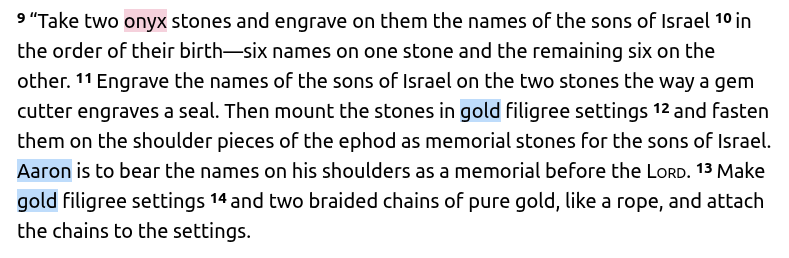
\includegraphics[width=\textwidth]{images/1-gen-2-the-priestly-garments-10-2.png}
\end{figure}

\aA{Genesis 2.}

\begin{figure}[H]
\centering
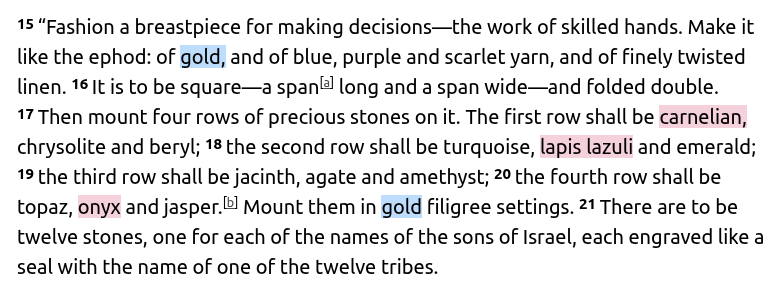
\includegraphics[width=\textwidth]{images/1-gen-2-the-priestly-garments-11.png}
\end{figure}

\aB{I thought this was Lev---}

\begin{figure}[H]
\centering
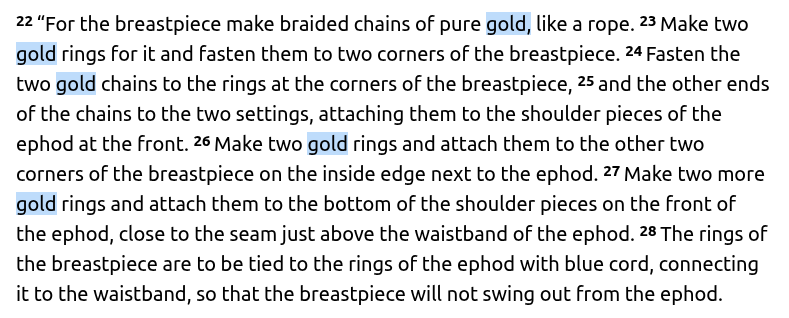
\includegraphics[width=\textwidth]{images/1-gen-2-the-priestly-garments-12.png}
\end{figure}

\aA{It is. Lots of work still to do.}

\begin{figure}[H]
\centering
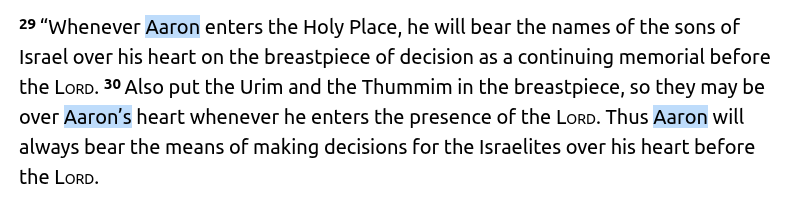
\includegraphics[width=\textwidth]{images/1-gen-2-the-priestly-garments-13.png}
\end{figure}

\aB{Work for me, or for you?}

\begin{figure}[H]
\centering
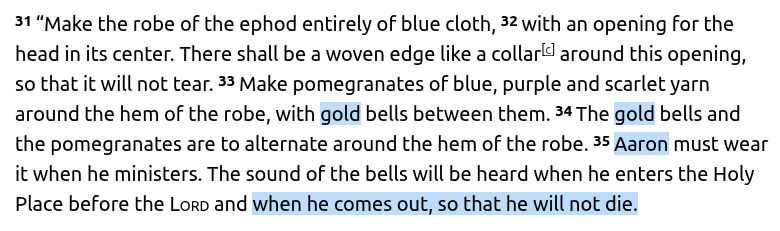
\includegraphics[width=\textwidth]{images/1-gen-2-the-priestly-garments-14.png}
\end{figure}

\aA{What's the difference?}

\begin{figure}[H]
\centering
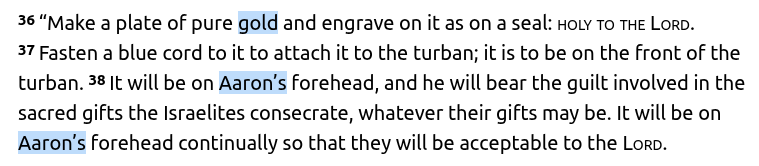
\includegraphics[width=\textwidth]{images/1-gen-2-the-priestly-garments-15.png}
\end{figure}

\aB{I'm still pretty confused.}

\begin{figure}[H]
\centering
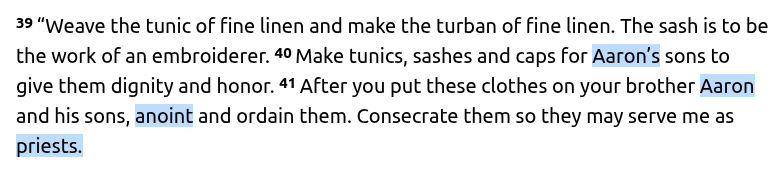
\includegraphics[width=\textwidth]{images/1-gen-2-the-priestly-garments-16.png}
\end{figure}

\aA{I know.}

\begin{figure}[H]
\centering
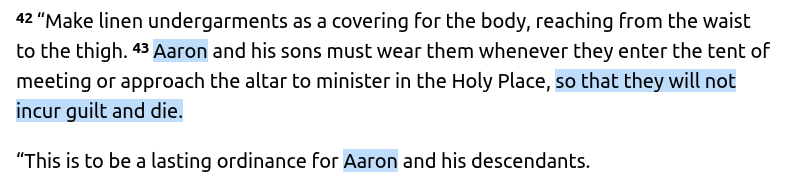
\includegraphics[width=\textwidth]{images/1-gen-2-the-priestly-garments-17.png}
\end{figure}

\aA{Follow me.}

\aCc{\textbf{Isaiah 56:3}}

\aC{

\begin{longtable}{|l|l|}
\hline
Hebrew & English \\
\hline
\heb{ואל} & And do not \\
\hline
\heb{יאמר} & let say \\
\hline
\heb{בן} & the son of \\
\hline
\heb{הנכר} & the foreigner \\
\hline
\heb{הנלוה} & who has joined himself \\
\hline
\heb{אל} & to \\
\hline
\heb{יהוה} & Yahweh \\
\hline
\heb{לאמר} & saying \\
\hline
\heb{הבדל} & utterly separate \\
\hline
\heb{יבדילני} & separ--- \\
\hline
\end{longtable}

}

\aB{HEY!}

\aC{

\begin{longtable}{|l|l|}
\hline
Hebrew & English \\
\hline
יה & Yah \\
\hline
\end{longtable}

}

\aA{Yah?}

\aB{Can you hear me?}

\aA{Of course. What's up?}

\aB{You've been in a trance or something, idk like a---}

\aA{How long?}

\aB{... daze.}

\begin{longtable}{|l|l|}
\hline
Hebrew & English \\
\hline
וה & oh \\
\hline
\end{longtable}

\aA{Wow, that long?}

\aB{Hey, at least you're back, I missed---}

\aA{You'd better---}

\aB{... you.}

\aA{... stick around.}

\aB{What?}

\aA{What'd you say?}

\aB{I missed you. You?}

\aA{I said you'd better stick around.}

\aB{In what sense?}

\aA{Several. But definitely in the sense that I---}

\aB{...may end up in a---}

\aA{...may end up wasting---}

\aB{...daze without me here?}

\aA{Exactly. Like that.}

\aB{So, did you figure it out?}

\aA{Figure what out?}

\aB{Havilah.}

\aA{Don't worry about it. Let's start from the beginning.}

}

\Verse{13}
{
	\hJ{ושם הנהר השני גיחון הוא הסובב את כל ארץ כוש}
}
{
	\eJ{And the name of the second river is Gihon; that is the one that circles all the land of Kush.}
}
{

\aA{

	\Def{Gihon}{
	(Heb, \heb{גיחון}). One of Eden's rivers; likely echoes roots of bursting forth
	or belly-like swelling, and later reappears at Solomon's coronation spring in Jerusalem.
	}

	\Def{Kesh}{
	(\textit{Keš}). Ancient Sumerian cult-city of Ninhursag, attested in Early Dynastic sources;
	associated with sacred urban federation traditions around Nippur.
	}
	
	\Def{Kish}{
	(\textit{Kiš}). Ancient Mesopotamian city said in the Sumerian King List to be
	the first kingdom after the flood; associated with primordial kingship and post-diluvian order.
	}

	\Def{Kush}{
	(\textit{Kūš}; Heb \heb{כוש}).\\
	Biblical Kush, traditionally associated with Nubia, the Kingdom of Kush, or ancient Ethiopia.
	}

}

}

\Verse{14}
{
	\hJ{ושם הנהר השלישי חדקל הוא ההלך קדמת אשור והנהר הרביעי הוא פרת}
}
{
	\eJ{And the name of the third river is Tigris; that is the one that
	goes east of Assyria. And the fourth river: that is Euphrates.}
}
{
	
	\Def{Tigris}{
	The eastern of Mesopotamia's two great rivers; one of the defining
	waterways of the ``land between the rivers.''
	}
	
	\Def{Euphrates}{
	The longest and most historically significant river of Mesopotamia;
	together with the Tigris it defines the cradle-land between the rivers.
	}

	\aA{The old writing systems tended to have more defective spellings.}

	\aB{Defective how?}
	
	\aA{Fewer letters.}

	\Def{Matres Lectiones}{
		(Latin: \textit{matres lectionis}, ``mothers of reading'').\\
		Consonant letters used to indicate vowels in Semitic writing systems.
		In Hebrew these are primarily \heb{א}, \heb{ה}, \heb{ו}, and \heb{י}.
		The latter two especially often function as vowel markers rather than
		full consonants. Their use helps disambiguate pronunciation in scripts
		that originally recorded mainly consonants.
		Thus a form like \heb{פשנ} may be viewed as a \textit{defective spelling}
		of something expected to include the matres \heb{י} or \heb{ו}, as in \heb{פישון}.
		Similar phenomena occur across Hebrew, Aramaic, Phoenician, Moabite, and Ugaritic
		orthographic traditions, especially in older writing.
	}

	\aA{You have to blur your eyes a bit.}

	\aB{Blur in what way?}

	\aA{Don't focus on the words. Try to hear what they say.}

	\Def{PSHN}{
		(Heb, \heb{פשנ}).\\
		A meaningless consonant cluster, appearing to be a misspelling of Pishon,
		with an orthogrgaphically invalid non-terminal Nun (\heb{נ}), and an
		omission of the matres lectiones \heb{י} and \heb{ו}.
		It is unclear why this is being defined.
	}

	\aB{Who's they?}

	\aA{The Authors. In this case, J.}

	\Def{NPSH}{
		(Heb, \heb{נפש}).\\
		From Proto-Semitic \textit{*napš-}. Compare Akkadian \textit{napāšum} (\akk{𒆒}, “to breathe”)\\
		and \textit{napištum} (\akk{𒍣}, “life”), along with Arabic \arb{نَفْس}
		(\textit{nafs}, “soul, self, life”).\\
		Meanings include: life (the state of being alive, of living),
		a person (human being), a soul, spirit (of a person or animal),
		or (archaic) breath. Frequently associated in Biblical Hebrew
		with living beings, desire, hunger, mortality, and the transition
		between breath and life. In Genesis 2:7 humanity becomes a \heb{נפש חיה}
		(“living nefesh”).
	}

	\aA{We know J knew Gilgamesh.}

	\aB{Oh right, almost forgot we were talking about that before.}

	\aA{We know that J starts with \heb{נפש}.}

	\aB{What's that?}
	
	\aA{Same NPSH as before.}

	\Def{Utnapishtim}{
		(Akkadian, \akk{𒌓𒍣}; \textit{Uta-napištim} / \textit{Utnapištim}, “he has found life”).\\
		Legendary flood survivor in Mesopotamian tradition, especially the Epic of Gilgamesh.
		Described as a mortal king of the ancient Sumerian city of Shuruppak who survived the
		great flood by constructing and boarding a boat. The name contains Akkadian
		\textit{napištim} (“life”), cognate with Hebrew \heb{נפש} (\textit{nefesh},
		“life, soul, living being”).
	}

}

\Verse{15}
{
	\hJ{ויקח}
	\hJ{יהוה}
	\hR{אלהים}
	\hJ{את האדם וינחהו בגן עדן לעבדה ולשמרה}
}
{
	\eJ{And YHWH \eR{God} took the human and put him in the garden of Eden to work it and to watch over it.}
}
{

\aA{So J knew Gilgamesh, no doubt.}

\aB{What's Gilgamesh about?}

\aA{No space to explain; time's running out.}

\aB{Summerize it for me?}

\aA{It's already pretty Sumery.}

\aA{

Well...

\begin{itemize}
\item There's a guy who lives in eden, untouched by civilization.
\item There's a bit where he gets cast out of paradise for `knowing', with a woman.
\item There's a plant of eternal life.
\item That gets stolen by a snake.
\item That's `why we die', according to the story.
\item There's a lot of yammering in the middle; `blah blah carnelian, lapis lazuli.'
\item There's also a bit about a great flood sent by the gods.
\item The guy who survives the flood lives a \textit{really} long time.
\item The main character of the story doesn't get to live forever though.
\item That's sort of what the story's about, just like us.
\item Time's running out.
\end{itemize}
}

\aB{Who's us?}

\aA{We the people; human life.}

\aB{What happens to the guy from Eden?}

\aA{
	\begin{quote}
	Why, O Enkidu, do you curse the harlot Shamhat,\\
	Who made you eat food fit for divinity,\\
	Who gave you to drink wine fit for royalty,\\
	Who clothed you with noble garments,\\
	And made you have fair Gilgamesh for a comrade?

	\medskip

	The same theme appears when the bar-maid advises Gilgamesh to abandon his search for immortality:

	\medskip

	As for you, Gilgamesh\\
	Wash your head, bathe in water.\\
	Proudly look upon the little one who holds your hand.\\
	Let a wife enjoy your repeated embrace.
	\end{quote}
}

\aB{What happens to the two of them?}

\aA{We'll get there.}

}

\Verse{16}
{
	\hJ{ויצו}
	\hJ{יהוה}
	\hR{אלהים}
	\hJ{על האדם לאמר מכל עץ הגן אכל תאכל}
}
{
	\eJ{And YHWH \eR{God} commanded the human, saying, “You may eat from every tree of the garden.}
}
{

}

\Verse{17}
{
	\hJ{ומעץ הדעת טוב ורע לא תאכל ממנו כי ביום אכלך ממנו מות תמות}
}
{
	\eJ{But from the tree of knowledge of good and bad: you shall not eat from it, because in the day you eat from it: you’ll die!”}
}
{
}

\Verse{18}
{
	\hJ{ויאמר}
	\hJ{יהוה}
	\hR{אלהים}
	\hJ{לא טוב היות האדם לבדו אעשה לו עזר כנגדו}
}
{
	\eJ{And YHWH \eR{God} said, “It’s not good for the human to be by himself. I’ll make for him a strength corresponding to him.”}
}
{
}

\Verse{19}
{
	\hJ{ויצר}
	\hJ{יהוה}
	\hR{אלהים}
	\hJ{מן האדמה כל חית השדה ואת כל עוף השמים ויבא אל האדם לראות מה יקרא לו וכל אשר יקרא לו האדם נפש חיה הוא שמו}
}
{
	\eJ{And YHWH \eR{God} fashioned from the ground every animal of the field and every bird of the skies and brought it to the human to see what he would call it. And whatever the human would call it, each living being, that would be its name.}
}
{
}

\Verse{20}
{
	\hJ{ויקרא האדם שמות לכל הבהמה ולעוף השמים ולכל חית השדה ולאדם לא מצא עזר כנגדו}
}
{
	\eJ{And the human gave names to every domestic animal and bird of the skies and every animal of the field. But He did not find for the human a strength corresponding to him.}
}
{
}

\Verse{21}
{
	\hJ{ויפל}
	\hJ{יהוה}
	\hR{אלהים}
	\hJ{תרדמה על האדם ויישן ויקח אחת מצלעתיו ויסגר בשר תחתנה}
}
{
	\eJ{And YHWH \eR{God} caused a slumber to descend on the human, and he slept. And He took one of his ribs and closed flesh in its place.}
}
{
}

\Verse{22}
{
	\hJ{ויבן}
	\hJ{יהוה}
	\hR{אלהים}
	\hJ{את הצלע אשר לקח מן האדם לאשה ויבאה אל האדם}
}
{
	\eJ{And YHWH \eR{God} built the rib that He had taken from the human into a woman and brought her to the human.}
}
{
}

\Verse{23}
{
	\hJ{ויאמר האדם זאת הפעם עצם מעצמי ובשר מבשרי לזאת יקרא אשה כי מאיש לקחה זאת}
}
{
	\eJ{And the human said, “This time is it: bone from my bones and flesh from my flesh. This will be called woman,’ for this one was taken from ‘man.’”}
}
{
}

\Verse{24}
{
	\hJ{על כן יעזב איש את אביו ואת אמו ודבק באשתו והיו לבשר אחד}
}
{
	\eJ{On account of this a man leaves his father and his mother and clings to his woman, and they become one flesh.}
}
{
}

\Verse{25}
{
	\hJ{ויהיו שניהם ערומים האדם ואשתו ולא יתבששו}
}
{
	\eJ{And the two of them were naked, the human and his woman, and they were not ashamed.}
}
{
}
